%----------------------------------------------------------------------
\section{Stochastic gradient descent for logistic regression}
\label{sec:logregsgd}

\index{stochastic gradient descent!logistic regression}
\index{minibatch!logistic regression}
The two optimisers of Section~\ref{sec:logregoptim} -- gradient descent and
Newton's method -- both touch every observation before they move the
parameters once.  For the few hundred points of the examples so far this is
of no consequence.  It becomes the whole story when $n$ is large, and
Section~\ref{sec:sgd} argued in general terms that the remedy is to update
on \emph{minibatches}: for a cost that is a sum over observations the
minibatch gradient is an unbiased estimate of the full one at a fraction of
the price, and the statistical accuracy worth having is reached after a few
passes over the data.  The cross entropy is such a sum, and logistic
regression is the simplest model on which the argument can be checked
rather than merely asserted.  We do so here, and then run the adaptive
methods of Chapter~\ref{chap:optim} on the same problem, so that when the
same loop reappears in Chapter~\ref{chap:nn} with a network in place of the
neuron, nothing about the optimiser will be new.

%......................................................................
\subsection{Minibatches and the per-observation gradient}
\label{sec:logregminibatch}

In the $1/n$ convention of the class of Section~\ref{sec:logregcode} the
cost is the mean of the per-observation costs of
Eq.~(\ref{eq:5-crossentropycompact}),
\begin{equation}
  C(\bm{\theta}) = \frac1n\sum_{i=1}^{n}c_i(\bm{\theta}),
  \qquad
  c_i(\bm{\theta}) = \ln\bigl(1+e^{z_i}\bigr)-y_iz_i,
  \qquad z_i=\bm{x}_i^{T}\bm{\theta},
  \label{eq:5-costmean}
\end{equation}
and each term has the gradient~(\ref{eq:5-gradone}),
$\nabla c_i=(p_i-y_i)\bm{x}_i$, which we read off the neuron of
Figure~\ref{fig:5-neuron}.  A minibatch $B$ of $M$ observations drawn
without replacement gives the estimate
\begin{equation}
  \bm{g}_B(\bm{\theta})
   = \frac1M\sum_{i\in B}(p_i-y_i)\,\bm{x}_i
   = \frac1M\,\bm{X}_B^{T}\bigl(\bm{p}_B-\bm{y}_B\bigr),
  \label{eq:5-minibatchgrad}
\end{equation}
where $\bm{X}_B$ holds the $M$ selected rows of the design matrix.  This is
Eq.~(\ref{eq:5-gradient}) restricted to the rows in $B$ and divided by $M$,
so the code that computes it is the code that computes the full gradient,
handed fewer rows.  By Eq.~(\ref{eq:4-minibatchvar}) it is unbiased,
$\mathbb{E}[\bm{g}_B]=\nabla C$, with a variance that scales as $1/M$; the
update
\begin{equation}
  \bm{\theta}_{t+1} = \bm{\theta}_t - \gamma_t\,\bm{g}_{B_t}(\bm{\theta}_t)
  \label{eq:5-sgdupdate}
\end{equation}
is Eq.~(\ref{eq:4-sgdupdate}) for the cross entropy, and with $M=1$ it is
the delta rule~(\ref{eq:5-deltarule}) applied to one observation at a
time.  One pass over the data, an \emph{epoch}, consists of $n/M$ such
updates, against a single update of gradient descent.

\paragraph{What an epoch costs, and what it buys.}
The count of Eq.~(\ref{eq:4-flops}) transfers directly: the minibatch
gradient~(\ref{eq:5-minibatchgrad}) is one matrix--vector product
$\bm{X}_B\bm{\theta}$, $M$ evaluations of the sigmoid and one product
$\bm{X}_B^{T}\bm{r}_B$, about $4Mp$ floating-point operations, so that an
epoch of SGD costs the same $4np$ as one step of gradient descent.  The
question is therefore how much each of the two buys per pass over the
data, and the two extremes are easy to state.  Gradient descent
descends at the rate set by the condition number of the Hessian,
Eq.~(\ref{eq:4-gdrate}), and needs of order $\kappa\ln(1/\epsilon)$ passes
to reach an excess cost $\epsilon$.  Stochastic gradient descent makes
$n/M$ moves per pass; early on, when the parameters are far from the
optimum, almost every one of them points downhill and the method covers in
one epoch what gradient descent covers in hundreds.  Late in the run the
minibatch noise takes over: at a constant learning rate the iterate does
not settle at the minimum but equilibrates in the cloud of
Eq.~(\ref{eq:4-sgdcloud}), of excess cost proportional to $\gamma/M$, and
only a decaying learning rate removes it.  The relevant accuracy is set by
statistics, as in Section~\ref{sec:sgd}.  The minimiser $\hat{\bm{\theta}}$
of the empirical cross entropy is the maximum-likelihood estimate of
Section~\ref{sec:maxlikelihood}, and the classical result on the likelihood
ratio says that $2n\,[C(\bm{\theta}_{\mathrm{true}})-C(\hat{\bm{\theta}})]$
is asymptotically $\chi^{2}$-distributed with $p$ degrees of freedom, so
the parameters that generated the data sit at an excess cost of about
$p/(2n)$ above the empirical minimum.  Optimising below that level chases
the noise of this particular sample; it is the analogue for the cross
entropy of the floor $\sigma^{2}p/n$ of Eq.~(\ref{eq:4-flopcompare}).

\paragraph{The learning rate of gradient descent.}
For the comparison to be fair, gradient descent must be given its best
constant learning rate, and logistic regression has a feature here that
least squares does not.  The Hessian $\bm{X}^{T}\bm{W}\bm{X}/n$ of
Eq.~(\ref{eq:5-hessian}) changes along the path, because the weights
$W_{ii}=p_i(1-p_i)$ do.  At the starting point $\bm{\theta}=\bm{0}$ every
$p_i$ equals $\tfrac12$, every weight equals its maximum $\tfrac14$, and
the stability bound~(\ref{eq:4-stability}) reads
\begin{equation}
  \gamma < \frac{2}{\lambda_{\max}\bigl(\bm{X}^{T}\bm{W}\bm{X}/n\bigr)}
   = \frac{8}{\lambda_{\max}\bigl(\bm{X}^{T}\bm{X}/n\bigr)}
  \qquad\text{at }\bm{\theta}=\bm{0},
  \label{eq:5-gdstability}
\end{equation}
the safe choice already quoted in Section~\ref{sec:logregoptim}.  As the
fit sharpens the weights shrink, the Hessian becomes smaller, and a larger
step would be admissible near the optimum -- but a step chosen for the
optimum overshoots at the start, where the curvature is largest.  A
constant learning rate must respect the largest curvature met along the
way, and Eq.~(\ref{eq:5-gdstability}) is it.

%......................................................................
\subsection{Gradient descent against SGD, measured}
\label{sec:logregsgdvsgd}

We construct a problem large enough for the difference to show and small
enough to run in seconds: $n=50\,000$ observations and $p=20$ parameters,
an intercept and nineteen standardised features with the same
autoregressive correlation of $0.9$ between neighbouring columns as in
Section~\ref{sec:sgd}, so that the design is strongly correlated.  The
labels are drawn as $y_i\sim\mathrm{Bernoulli}(\sigma(\bm{x}_i^{T}
\bm{\theta}_{\mathrm{true}}))$ from a known parameter vector; $40\%$ of
them are ones, and even the true parameters classify only $76.7\%$ of the
points correctly, because the classes overlap.  Newton's method of
Section~\ref{sec:logregoptim} converges in seven iterations to the reference
value $C(\hat{\bm{\theta}})=0.47624$, against which every excess cost below
is measured; the Hessian there has condition number $\kappa=173$, and
$\lambda_{\max}(\bm{X}^{T}\bm{X}/n)=10.9$ gives the learning rate
$\gamma=0.73$ of Eq.~(\ref{eq:5-gdstability}) for gradient descent.  The
excess cost of $\bm{\theta}_{\mathrm{true}}$ is $2.7\times10^{-4}$, close
to the $p/(2n)=2\times10^{-4}$ of the $\chi^{2}$ argument; this is the
dotted line in Figure~\ref{fig:5-sgdvsgd}, and the level below which
further optimisation is pointless.

\begin{figure}[htbp]
\centering
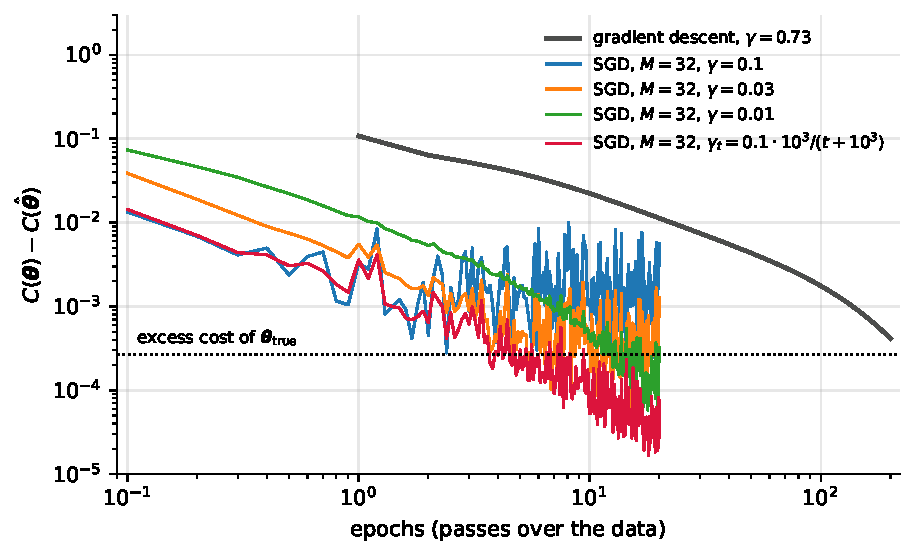
\includegraphics[width=0.8\textwidth]{BookFigures/chapter05_logistic_regression/logreg_sgd_vs_gd}
\caption{Excess cross entropy $C(\bm{\theta})-C(\hat{\bm{\theta}})$ against
passes over the data for the logistic regression problem of
Section~\ref{sec:logregsgdvsgd} ($n=50\,000$, $p=20$, $\kappa=173$).
Gradient descent uses the learning rate~(\ref{eq:5-gdstability}); the SGD
runs use minibatches of $M=32$, the cost being recorded ten times per
epoch, at three constant learning rates and with the decaying schedule
$\gamma_t=0.1\cdot10^{3}/(t+10^{3})$.  The dotted line is the excess cost of
the parameters that generated the data, about $p/(2n)$.  After a single epoch
every SGD run is where gradient descent is after twenty.  The constant-rate
runs then equilibrate in a cloud whose size grows with $\gamma$, as
Eq.~(\ref{eq:4-sgdcloud}) predicts, the smallest rate reaching within
twenty epochs the level gradient descent needs two hundred for; only the
decaying schedule continues downwards.}
\label{fig:5-sgdvsgd}
\end{figure}

Figure~\ref{fig:5-sgdvsgd} and the first block of the output below tell
the same story.  Gradient descent reduces the excess cost to
$1.1\times10^{-1}$ after one pass, $3.9\times10^{-2}$ after five,
$1.1\times10^{-2}$ after twenty and reaches $4.1\times10^{-4}$, about the
statistical floor, only after $200$ passes; the slow, steady slope is the
rate $(1-2/\kappa)^{k}$ of a problem with $\kappa=173$.  Stochastic gradient
descent with $M=32$ and $\gamma=0.01$ is at $1.8\times10^{-3}$ after five
passes and $3.2\times10^{-4}$ after twenty, so that five epochs of SGD are
worth about a hundred of gradient descent and twenty are worth two
hundred.  Since an epoch of either costs the same $4np$ operations, this is
a factor of ten to twenty in computation, obtained without tuning anything.
With the decaying schedule the excess is $3.0\times10^{-4}$ after five
epochs and $2.8\times10^{-5}$ after twenty -- an order of magnitude below
the floor, and still falling.  The larger constant rates show the other
side of the coin: $\gamma=0.1$ is fastest in the first epoch but then
oscillates in a band an order of magnitude wide, and the band for
$\gamma=0.03$ is narrower by about the ratio of the learning rates, as
Eq.~(\ref{eq:4-sgdcloud}) says it should be.  One more column of the output
deserves attention: the accuracy.  Gradient descent classifies $68.8\%$ of
the training points correctly after one pass, $74.3\%$ after five and
$76.1\%$ after twenty, while both SGD runs of the listing are at $76.7\%$
after twenty epochs, the accuracy of the true parameters.  The accuracy
saturates long before the cost does -- an excess cost of $10^{-3}$ already
gives an accuracy within half a percent of the best possible -- which is
why, for classification, a few epochs of SGD are usually all that is ever
run.

%......................................................................
\subsection{AdaGrad, RMSProp and Adam on the same problem}
\label{sec:logregadaptive}

\index{AdaGrad!logistic regression}\index{RMSProp!logistic regression}
\index{Adam!logistic regression}
The three adaptive methods of Sections~\ref{sec:adagrad} to~\ref{sec:adam}
replace the single learning rate of Eq.~(\ref{eq:5-sgdupdate}) by one per
parameter, obtained from a running average of the squared minibatch
gradients: AdaGrad accumulates the squares, Eq.~(\ref{eq:4-adagrad}),
RMSProp averages them with exponential forgetting,
Eq.~(\ref{eq:4-rmsprop}), and Adam adds a momentum-like average of the
gradient itself with bias corrections, Eq.~(\ref{eq:4-adam}).  All three
are the diagonally preconditioned iteration of Eq.~(\ref{eq:4-precond}),
and Chapter~\ref{chap:optim} drew two conclusions from that form: the
preconditioner equalises the curvature \emph{along the coordinate axes} and
therefore undoes any difference in the scales of the features, but it can
do nothing about curvature caused by correlation between them, which is not
diagonal.  Logistic regression lets us test both conclusions with one
switch, because the data of the previous subsection come standardised, and
we may unstandardise them.

Figure~\ref{fig:5-adaptive} shows the four stochastic methods -- plain SGD
and the three adaptive ones, minibatches of $32$ throughout -- and gradient
descent, first on the standardised features of Figure~\ref{fig:5-sgdvsgd}
and then on the same data with each feature column multiplied by a fixed
random factor between $0.1$ and $10$, the kind of disparity in units that
raw data carry.  For each method the constant learning rate was chosen from
a grid of five values a factor of $\sqrt{10}$ apart as the one with the
smallest mean excess cost over epochs $15$ to $20$; the listing below runs
the winners, and Table~\ref{tab:5-sgdcompare} collects the numbers.

\begin{figure}[htbp]
\centering
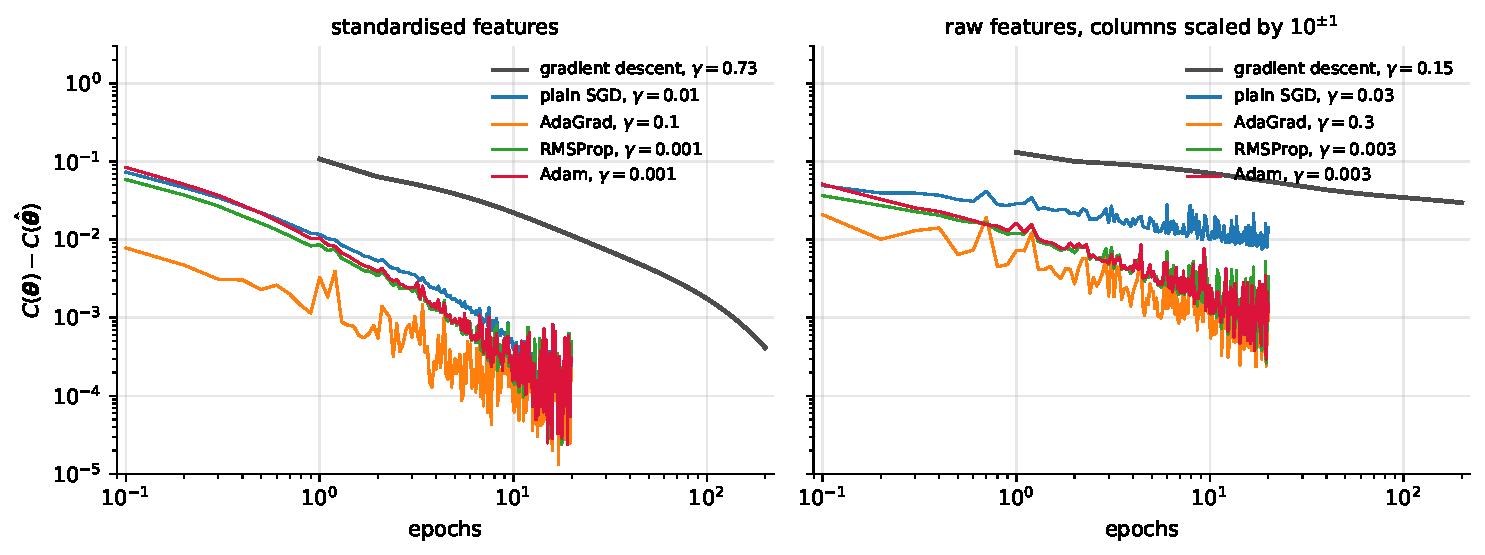
\includegraphics[width=0.98\textwidth]{BookFigures/chapter05_logistic_regression/logreg_adaptive}
\caption{Plain SGD, AdaGrad, RMSProp and Adam, all with $M=32$ and each at
the best of five constant learning rates, against gradient descent at the
learning rate~(\ref{eq:5-gdstability}), on the logistic regression problem
of Section~\ref{sec:logregsgdvsgd}.  Left: standardised features,
$\kappa=173$.  Right: the same data with each feature column multiplied by
a random factor between $0.1$ and $10$, which raises the condition number
of the Hessian at the optimum to $4.4\times10^{4}$ and the excess cost of
the two plain-gradient methods by nearly two orders of magnitude, while the
three adaptive methods lose less than one.  On standardised
features the four stochastic methods are indistinguishable after ten
epochs.}
\label{fig:5-adaptive}
\end{figure}

\begin{table}[htbp]
\centering
\caption{Excess cross entropy $C(\bm{\theta})-C(\hat{\bm{\theta}})$ and
training accuracy for the methods of Figure~\ref{fig:5-adaptive}, from the
output of the listing below.  Gradient descent is listed after $200$ epochs,
the stochastic methods after $20$; the column ``mean'' averages the excess
cost at the ends of epochs $15$ to $20$, which smooths the fluctuations of
the constant-rate runs.  The excess cost of the parameters that generated
the data is $2.7\times10^{-4}$ in both cases.}
\label{tab:5-sgdcompare}
\renewcommand{\arraystretch}{1.2}
\setlength{\tabcolsep}{6pt}
\begin{tabular}{lrrrr}
\toprule
\textbf{Method} & $\gamma$ & \textbf{excess, 5 epochs} & \textbf{mean, 15--20} & \textbf{accuracy}\\
\midrule
\multicolumn{5}{l}{\emph{standardised features, $\kappa=173$}}\\
gradient descent (200 epochs) & $0.73$  & $3.9\times10^{-2}$ & $4.1\times10^{-4}$ & $0.7671$\\
SGD                           & $0.01$  & $1.8\times10^{-3}$ & $1.9\times10^{-4}$ & $0.7666$\\
SGD, $\gamma_t=0.1\cdot10^{3}/(t+10^{3})$ & $0.1$ & $3.0\times10^{-4}$ & $5.1\times10^{-5}$ & $0.7671$\\
AdaGrad                       & $0.1$   & $3.0\times10^{-4}$ & $1.3\times10^{-4}$ & $0.7670$\\
RMSProp                       & $0.001$ & $9.4\times10^{-4}$ & $2.3\times10^{-4}$ & $0.7663$\\
Adam                          & $0.001$ & $9.7\times10^{-4}$ & $2.2\times10^{-4}$ & $0.7666$\\
\midrule
\multicolumn{5}{l}{\emph{raw features, $\kappa=4.4\times10^{4}$}}\\
gradient descent (200 epochs) & $0.15$  & $8.6\times10^{-2}$ & $3.0\times10^{-2}$ & $0.7471$\\
SGD                           & $0.03$  & $1.8\times10^{-2}$ & $1.2\times10^{-2}$ & $0.7585$\\
AdaGrad                       & $0.3$   & $2.2\times10^{-3}$ & $9.4\times10^{-4}$ & $0.7657$\\
RMSProp                       & $0.003$ & $3.6\times10^{-3}$ & $1.7\times10^{-3}$ & $0.7647$\\
Adam                          & $0.003$ & $3.3\times10^{-3}$ & $1.3\times10^{-3}$ & $0.7656$\\
\bottomrule
\end{tabular}
\end{table}

Three things stand out.  First, on standardised features the adaptive
methods bring nothing that plain SGD does not already have: after ten
epochs all four sit at the statistical floor, within a factor of two of
one another, and the ordering among them changes from epoch to epoch with
the noise.  The condition number $\kappa=173$ of this problem comes from the
correlation between the columns, not from their scales, and a diagonal
preconditioner cannot see it.  Second, on the raw features the picture
changes completely.  Gradient descent, forced by Eq.~(\ref{eq:5-gdstability})
to a learning rate five times smaller, is at an excess cost of
$3\times10^{-2}$ after $200$ epochs, worse than SGD on the standardised
data was after one; plain SGD is at $10^{-2}$ after twenty epochs, with a
training accuracy nearly a full percent below the optimum, and no constant learning
rate does better, since the step that suits the columns scaled by $10$
crawls on those scaled by $0.1$ and the reverse diverges.  The three
adaptive methods recover an order of magnitude of that loss, ending at
$10^{-3}$ with accuracies within a quarter of a percent of the optimum, because their
per-parameter learning rates absorb the column scales, as the scale
invariance of Section~\ref{sec:adaptive} says they must.  They do not
recover it all -- the remaining factor of five to ten against the
standardised case is the correlation, which survives rescaling.  Third, the
learning rates that work differ by two orders of magnitude between the
methods, and this is not a matter of tuning but of units: for plain SGD
$\gamma$ multiplies a gradient, while for RMSProp and Adam the update
$\gamma\,\bm{g}/\sqrt{\bm{v}}$ has the size of $\gamma$ itself in every
coordinate (Section~\ref{sec:adam}), so $\gamma$ is a step length in
parameter space and $10^{-3}$ is a sensible value; AdaGrad's ever-growing
accumulator shrinks its steps as $1/\sqrt{t}$, Eq.~(\ref{eq:4-adagradschedule}),
which is why it tolerates, and needs, a rate a hundred times larger.

The listing runs every method of Table~\ref{tab:5-sgdcompare}.  The
optimiser is the step function of Section~\ref{sec:adaptivecode}; the data
loop knows nothing about which method it is driving, and the gradient
function is the same for a minibatch as for the full data, which is all
that Eq.~(\ref{eq:5-minibatchgrad}) requires.

\begin{Python}{}
import numpy as np

def sigmoid(t):                                   # the stable form of Section 5.7
    a = np.exp(-np.abs(t))
    return np.where(t >= 0, 1.0 / (1.0 + a), a / (1.0 + a))

def make_data(n=50_000, p=20, rho=0.9, seed=2026):
    """AR(1)-correlated standardised features, Bernoulli labels from a known theta."""
    rng = np.random.default_rng(seed)
    z = rng.normal(size=(n, p - 1)); xc = np.empty_like(z); xc[:, 0] = z[:, 0]
    for j in range(1, p - 1):
        xc[:, j] = rho * xc[:, j - 1] + np.sqrt(1 - rho**2) * z[:, j]
    xc = (xc - xc.mean(0)) / xc.std(0)
    X = np.column_stack([np.ones(n), xc])
    theta_true = 0.5 * rng.normal(size=p)
    y = (rng.random(n) < sigmoid(X @ theta_true)).astype(float)
    scales = np.concatenate([[1.0], 10.0**rng.uniform(-1, 1, p - 1)])   # "raw" units
    return X, y, theta_true, scales

def cost(X, y, theta):                            # mean cross entropy, Eq. (5.costmean)
    z = X @ theta
    return np.mean(np.logaddexp(0.0, z) - y * z)

def gradient(X, y, theta):                        # Eq. (5.minibatchgrad) on whatever rows it is given
    return X.T @ (sigmoid(X @ theta) - y) / X.shape[0]

def optimiser_step(method, theta, g, state, t, gamma, rho=0.99,
                   beta1=0.9, beta2=0.999, eps=1e-8):
    """The step function of Section 4.12, without momentum."""
    if method == "plain":
        return theta - gamma * g
    if method == "adagrad":                                             # Eq. (4.adagrad)
        state["r"] = r = state.get("r", 0.0) + g * g
        return theta - gamma * g / (np.sqrt(r) + eps)
    if method == "rmsprop":                                             # Eq. (4.rmsprop)
        state["r"] = r = rho * state.get("r", 0.0) + (1 - rho) * g * g
        return theta - gamma * g / (np.sqrt(r) + eps)
    if method == "adam":                                                # Eq. (4.adam)
        state["m"] = m = beta1 * state.get("m", 0.0) + (1 - beta1) * g
        state["r"] = r = beta2 * state.get("r", 0.0) + (1 - beta2) * g * g
        return theta - gamma * (m / (1 - beta1**t)) / (np.sqrt(r / (1 - beta2**t)) + eps)

def train(X, y, method, gamma, M=None, epochs=20, t0=None, seed=1):
    """Minibatch training loop; M=None is full-batch gradient descent.  Returns theta after each epoch."""
    n, p = X.shape; M = n if M is None else M
    rng = np.random.default_rng(seed); theta = np.zeros(p); state = {}; t = 0; history = []
    for epoch in range(epochs):
        idx = rng.permutation(n)
        for k in range(0, n, M):                                        # one epoch = n/M updates
            t += 1
            gam = gamma if t0 is None else gamma * t0 / (t + t0)        # optional decay, Eq. (4.sgdcloud)
            b = idx[k:k + M]
            theta = optimiser_step(method, theta, gradient(X[b], y[b], theta), state, t, gam)
        history.append(theta.copy())
    return history

X, y, theta_true, scales = make_data()
for label, Xd in (("standardised", X), ("raw", X * scales)):
    # the reference: Newton-Raphson to machine precision
    th = np.zeros(X.shape[1])
    for _ in range(50):
        pr = sigmoid(Xd @ th); H = Xd.T @ ((pr * (1 - pr))[:, None] * Xd) / len(y)
        step = np.linalg.solve(H, Xd.T @ (pr - y) / len(y)); th -= step
        if np.linalg.norm(step) < 1e-12: break
    c_star = cost(Xd, y, th)
    gamma_gd = 8.0 / np.linalg.eigvalsh(Xd.T @ Xd / len(y)).max()      # Eq. (5.gdstability)
    runs = [("GD, 200 epochs", dict(method="plain", gamma=gamma_gd, epochs=200))]
    if label == "standardised":
        runs += [("SGD", dict(method="plain", gamma=0.01, M=32)),
                 ("SGD, decaying", dict(method="plain", gamma=0.1, M=32, t0=1000.0)),
                 ("AdaGrad", dict(method="adagrad", gamma=0.1, M=32)),
                 ("RMSProp", dict(method="rmsprop", gamma=0.001, M=32)),
                 ("Adam", dict(method="adam", gamma=0.001, M=32))]
    else:
        runs += [("SGD", dict(method="plain", gamma=0.03, M=32)),
                 ("AdaGrad", dict(method="adagrad", gamma=0.3, M=32)),
                 ("RMSProp", dict(method="rmsprop", gamma=0.003, M=32)),
                 ("Adam", dict(method="adam", gamma=0.003, M=32))]
    print(f"{label} features: C* = {c_star:.5f}, excess of theta_true {cost(Xd, y, theta_true / (scales if label == 'raw' else 1)) - c_star:.1e}")
    print(f"  {'method':16s} gamma    excess after 1 / 5 / 20 epochs   mean 15-20   accuracy")
    for name, kw in runs:
        hist = train(Xd, y, **kw); ex = np.array([cost(Xd, y, th) - c_star for th in hist])
        last = ex[-1] if len(ex) > 20 else ex[14:].mean()
        e20 = ex[199] if len(ex) > 20 else ex[19]
        acc = np.mean((Xd @ hist[-1] > 0) == y)
        print(f"  {name:16s} {kw['gamma']:<7.3g}  {ex[0]:.1e} / {ex[4]:.1e} / {e20:.1e}      {last:.1e}     {acc:.4f}")
\end{Python}

\begin{Python}{}
standardised features: C* = 0.47624, excess of theta_true 2.7e-04
  method           gamma    excess after 1 / 5 / 20 epochs   mean 15-20   accuracy
  GD, 200 epochs   0.734    1.1e-01 / 3.9e-02 / 4.1e-04      4.1e-04     0.7671
  SGD              0.01     1.2e-02 / 1.8e-03 / 3.2e-04      1.9e-04     0.7666
  SGD, decaying    0.1      3.6e-03 / 3.0e-04 / 2.8e-05      5.1e-05     0.7671
  AdaGrad          0.1      3.3e-03 / 3.0e-04 / 2.2e-04      1.3e-04     0.7670
  RMSProp          0.001    8.7e-03 / 9.4e-04 / 4.9e-04      2.3e-04     0.7663
  Adam             0.001    1.0e-02 / 9.7e-04 / 2.8e-04      2.2e-04     0.7666
raw features: C* = 0.47624, excess of theta_true 2.7e-04
  method           gamma    excess after 1 / 5 / 20 epochs   mean 15-20   accuracy
  GD, 200 epochs   0.148    1.3e-01 / 8.6e-02 / 3.0e-02      3.0e-02     0.7471
  SGD              0.03     2.9e-02 / 1.8e-02 / 1.4e-02      1.2e-02     0.7585
  AdaGrad          0.3      7.3e-03 / 2.2e-03 / 1.8e-03      9.4e-04     0.7657
  RMSProp          0.003    1.2e-02 / 3.6e-03 / 3.4e-03      1.7e-03     0.7647
  Adam             0.003    1.6e-02 / 3.3e-03 / 1.5e-03      1.3e-03     0.7656
\end{Python}

For the gradient-descent rows the column ``20 epochs'' holds the value
after $200$; the raw-feature reference $C^{*}$ is the standardised one, as
it must be, since rescaling the columns rescales the parameters and
nothing else, Section~\ref{sec:adaptive}.  The whole run takes a few
seconds, and changing the loss, the minibatch size or the optimiser is one
line each -- the loop is the one that will train every network in this
book.

\begin{notebox}
\textbf{Machine learning connection.}  The recommendation that falls out of
Table~\ref{tab:5-sgdcompare} is the one every practitioner follows:
standardise the features, as Section~\ref{sec:scalingintercept} advised on
other grounds, use minibatches, and reach for Adam or RMSProp when the
scales cannot be controlled -- in a neural network the inputs to the inner
layers are activations whose scales are set by the training itself, and
that is where the adaptive methods earn their keep.  For logistic
regression itself, \texttt{scikit-learn}'s \texttt{SGDClassifier} with
\texttt{loss="log\_loss"} is Eq.~(\ref{eq:5-sgdupdate}) with a decaying
learning rate and an $\ell_2$ penalty, and its \texttt{partial\_fit} method
is the minibatch loop of the listing exposed to the user; its default
\texttt{LogisticRegression} class, by contrast, is the Newton-type
\texttt{lbfgs} of Section~\ref{sec:logregoptim}, the right choice whenever
the data fit in memory and $p$ is modest.  The dividing line between the
two is the one drawn in Section~\ref{sec:newtoncompete}, now with a
measured example on each side of it.
\end{notebox}

